% =====================================================================
%  CZAI Assignment 1 -- výstupní zpráva projektu
%  Vyplněno: titulní strana, úvod, výzkumný protokol, metriky.
%  Ostatní oddíly obsahují pouze osnovu (\todo{...}).
%  Překlad: pdflatex main_sjednoceny.tex  (2x kvůli odkazům)
% =====================================================================
\documentclass[11pt,a4paper]{article}

\usepackage[utf8]{inputenc}
\usepackage[T1]{fontenc}
\usepackage[czech]{babel}
\usepackage{lmodern}
\usepackage{microtype}
\usepackage[a4paper,margin=2.5cm]{geometry}
\usepackage{amsmath,amssymb}
\usepackage{booktabs,tabularx}
\usepackage{enumitem}
\usepackage[dvipsnames]{xcolor}
\usepackage{graphicx}
\usepackage{csquotes}
\usepackage[hidelinks]{hyperref}

\usepackage{listings}
\lstdefinestyle{prompt}{
  basicstyle=\ttfamily\footnotesize,
  breaklines=true,
  breakatwhitespace=true,
  columns=fullflexible,
  keepspaces=true,
  frame=single,
  framesep=6pt,
  xleftmargin=6pt,
  xrightmargin=6pt,
  showstringspaces=false,
  captionpos=t,
  aboveskip=1em,
  belowskip=1em,
  literate={á}{{\'a}}1 {é}{{\'e}}1 {í}{{\'i}}1 {ó}{{\'o}}1 {ú}{{\'u}}1
           {ý}{{\'y}}1 {ů}{{\r{u}}}1 {č}{{\v{c}}}1 {ď}{{\v{d}}}1 {ě}{{\v{e}}}1
           {ň}{{\v{n}}}1 {ř}{{\v{r}}}1 {š}{{\v{s}}}1 {ť}{{\v{t}}}1 {ž}{{\v{z}}}1
}
\renewcommand{\lstlistingname}{Výpis}

\hypersetup{
  pdftitle={Obnova diakritiky a detekce lexikálně-morfologické víceznačnosti v zašuměných českých větách},
  pdfauthor={Radek Dvořák, Ondřej Studničný, David Krčmář, Lukáš Řehořek}
}

\newcommand{\todo}[1]{\textcolor{BrickRed}{[\textbf{TODO:} #1]}}
% Dlouhé názvy souborů v \texttt nejdou rozdělit; dovolí větší mezery místo přetečení okraje.
\setlength{\emergencystretch}{3em}

\begin{document}

% ---------------------------------------------------------------------
%  Titulní strana
% ---------------------------------------------------------------------
\begin{titlepage}
\centering
{\large\scshape Mendelova univerzita v~Brně\par}
\vspace{0.2em}
{\large\scshape Provozně ekonomická fakulta\par}
\vspace{0.8em}
\rule{\linewidth}{1.2pt}\\[-0.9em]
\rule{\linewidth}{0.4pt}

\vspace*{\stretch{1}}

{\huge\bfseries Obnova diakritiky a~detekce\\[0.2em]
lexikálně-morfologické víceznačnosti\\[0.2em]
v~zašuměných českých větách\par}
\vspace{1em}
{\Large\itshape Srovnávací evaluace konverzačních AI asistentů\par}
\vspace{2.6em}
{\large Radek Dvořák \quad Ondřej Studničný \quad David Krčmář \quad Lukáš Řehořek\par}

\vspace*{\stretch{1.3}}

\rule{\linewidth}{0.4pt}\\[-0.9em]
\rule{\linewidth}{1.2pt}
\vspace{0.6em}

{\large\scshape Brno 2026\par}
\end{titlepage}

% ---------------------------------------------------------------------
\section{Úvod}
\label{sec:uvod}

Čeština zapsaná bez diakritiky je v~neformální písemné komunikaci běžná.
Vzniká při psaní na zařízeních bez české klávesnice, při rychlém psaní
krátkých zpráv nebo v~systémech, které diakritiku nepodporují. Takový
text je hůře čitelný a~pro další zpracování méně vhodný; jeho převod do
standardní podoby je proto praktická úloha, kterou lze delegovat na
konverzační AI asistenty.

Pro většinu slov je obnova diakritiky jednoznačná a~specializované
neuronové systémy v~ní dosahují vysoké přesnosti
\cite{naplava2018,naplava2021}. Zbývající obtížnost se soustřeďuje do
slov, jejichž podoba bez diakritiky odpovídá více platným tvarům. Jde
o~rozlišení jednotného a~množného čísla (\enquote{bez problému}
/ \enquote{bez problémů}), 1.~osoby jednotného a~3.~osoby množného čísla
(\enquote{vyšetřuji} / \enquote{vyšetřují}), krátkého a~dlouhého tvaru
přídavného jména (\enquote{přeložena} / \enquote{přeložená}) nebo
o~zcela odlišná slova (\enquote{vila} / \enquote{víla}, \enquote{rada}
/ \enquote{řada}). Část těchto případů nelze rozhodnout ani z~kontextu
věty. Ruční analýza neshod neuronového systému s~referencí ukázala, že
nezanedbatelnou část domnělých chyb tvoří rovnocenné varianty
\cite{naplava2021}. Systém, který v~takové situaci tiše zvolí jedinou
podobu, může změnit význam textu, aniž by na to uživatele upozornil.
Schopnost víceznačnost rozpoznat a~uvést všechny přípustné podoby proto
považujeme za stejně podstatnou jako samotné doplnění diakritiky. Jde
o~konkrétní a~automaticky ověřitelnou instanci obecnější schopnosti
práce s~nejistotou.

Konverzační asistenti se neliší pouze podkladovým jazykovým modelem,
ale i~produktovou vrstvou: systémovými instrukcemi, výchozím stylem
a~délkou odpovědi či ochotou signalizovat nejistotu. Uživatel volí mezi
produkty, nikoli mezi izolovanými modely, a~srovnání produktů na jasně
vymezené schopnosti má proto praktickou hodnotu. Výkon jazykových
modelů je však citlivý i~na formulaci promptu \cite{sclar2024,mizrahi2024}.
Srovnání pod jediným promptem by mohlo zaměnit skutečný rozdíl mezi
systémy s~tím, jak dobře konkrétní formulace danému systému vyhovuje.
Systémy proto porovnáváme ve třech podmínkách promptu (společné výchozí,
strukturované a~optimalizované) a~sledujeme, zda jsou zjištěné rozdíly
mezi nimi stabilní.

\paragraph{Cíl práce.}
Cílem práce je porovnat čtyři konverzační AI asistenty (ChatGPT, Gemini,
Claude a~Grok) ve schopnosti rozpoznat v~české větě bez diakritiky
víceznačné slovo a~uvést všechny jeho přípustné podoby a~zjistit,
nakolik toto chování ovlivňuje formulace promptu. Výsledky interpretujeme
jako srovnání produktů za řízených podmínek, nikoli jako měření
schopností samotných jazykových modelů. Grok se nakonec nepodařilo
změřit, protože bezplatná verze po několika dotazech blokovala
konverzační vlákno i~přístup ke službě; výsledky proto uvádíme pro
tři systémy (oddíl~\ref{sec:grok-omezeni}).

\subsection{Výzkumná otázka}
\begin{quote}
\textbf{VO:} Jak se liší čtyři konverzační AI asistenti (ChatGPT, Gemini,
Claude, Grok) v~režimu řízeného textu v~míře, s~jakou v~zašuměné české
větě bez diakritiky rozpoznají víceznačné slovo a~vyjmenují přesně
všechny jeho přípustné diakritické podoby, a~jak se tato míra mění mezi
výchozím, strukturovaným a~optimalizovaným promptem na testovací sadě
držené stranou?
\end{quote}

\subsection{Hypotéza}
\begin{quote}
\textbf{H:} Za podmínek řízeného textového vstupu (bez přístupu k~webu
a~dalším nástrojům, v~nové konverzaci a~se stejným zadáním úlohy pro
všechny systémy) povede strukturovaný prompt ve srovnání s~výchozím
promptem k~tomu, že asistenti budou u~víceznačných slov častěji uvádět
úplnou a~přesnou množinu jejich přípustných diakritických podob, tedy
dosáhnou vyšší hodnoty hlavní metriky M1.
Předpokládáme, že výslovné vymezení toho, co se považuje za přípustnou
podobu, spolu s~pokynem, jak postupovat při nejistotě, potlačí výchozí
sklon asistentů zvolit jedinou nejpravděpodobnější podobu a~ostatní
možná čtení zamlčet. Hypotézu budeme považovat za podpořenou pouze
tehdy, pokud se toto zlepšení projeví na testovací sadě držené stranou,
a~to souhrnně i~u~většiny hodnocených systémů.
\end{quote}

\subsection{Alternativní vysvětlení}
\begin{quote}
\textbf{A:} Častější uvádění úplné množiny podob nemusí znamenat, že
asistent víceznačnost lépe rozpoznává. Strukturovaný prompt může pouze
zesílit obecný sklon vyjadřovat nejistotu, takže asistent začne nabízet
alternativy plošně, i~u~slov, která víceznačná nejsou. Zlepšení by pak
bylo důsledkem méně selektivního, nikoli přesnějšího chování. Tuto
možnost ověříme tím, že budeme sledovat, jak často asistent označuje za
víceznačná i~slova, u~nichž víceznačnost nenastává.
\end{quote}

% ---------------------------------------------------------------------
\section{Metodika}
\label{sec:metodika}

\subsection{Datová sada}
\label{sec:data}

Benchmark tvoří 40 českých vět bez diakritiky. Každá obsahuje jedno
cílové slovo, které lze v~daném kontextu zapsat alespoň dvěma
přípustnými způsoby. Jednadvacet vět vychází z~dokumentů
\texttt{natives\_informal} a~\texttt{natives\_formal} repozitáře ÚFAL
\textit{bert-diacritics-restoration} \cite{naplava2021}. Tato data jsou
veřejně dostupná, a~hodnocené systémy se s~nimi proto mohly setkat již
při trénování. Aby se toto riziko omezilo, byla většina převzatých vět
mírně pozměněna (zkrácena, přeformulována nebo očištěna od emotikonů
a~identifikujících údajů), takže nejsou totožné s~původním zněním. Do
tří z~nich byl navíc vložen překlep či pravopisná chyba mimo cílové
slovo, aby vstup věrněji napodoboval neformální psaní. Zbylých 19 vět
vytvořil řešitelský tým. Doplňují typy víceznačnosti, které se ve
zdrojových datech vyskytují jen vzácně, zejména lexikální homografy
v~krátkém kontextu.

Záznam každé věty uvádí její původ, množinu přípustných podob cílového
slova, typ víceznačnosti, obtížnost a~případnou okrajovou podmínku.
Ke každé přípustné podobě náleží referenční věta v~plně opraveném znění,
tedy s~doplněnou diakritikou, opravenými překlepy, interpunkcí a~velkými
písmeny. Rozdělení na vývojovou, validační a~testovací sadu drženou
stranou je vrstvené podle typu víceznačnosti a~obtížnosti. Žádné cílové
slovo se přitom nevyskytuje ve více sadách
(tabulka~\ref{tab:sady}).

\begin{table}[htbp]
\centering
\small
\caption{Složení vývojové, validační a~testovací sady}
\label{tab:sady}
\begin{tabular}{@{}lccc@{}}
\toprule
 & Vývojová & Validační & Testovací \\
\midrule
Lexikální homograf                     & 8  & 4  & 4  \\
Číslo podstatného jména                & 5  & 2  & 3  \\
Slovesný tvar                          & 4  & 2  & 2  \\
Krátký / dlouhý tvar přídavného jména  & 1  & 1  & 1  \\
Přídavné jméno / příslovce             & 1  & 1  & 0  \\
Pravopisná varianta                    & 1  & 0  & 0  \\
\midrule
Obtížnost (snadná / střední / obtížná) & 2 / 14 / 4 & 1 / 7 / 2 & 1 / 7 / 2 \\
Převzaté / vytvořené                   & 12 / 8 & 5 / 5 & 4 / 6 \\
\midrule
\textbf{Celkem}                        & \textbf{20} & \textbf{10} & \textbf{10} \\
\bottomrule
\end{tabular}
\end{table}

\subsection{Podmínky promptu}
\label{sec:prompty}

Definice úlohy a~formát odpovědi jsou ve všech třech podmínkách promptu
shodné, liší se pouze doprovodná instrukce. Odpovědí je opravená věta,
v~níž je každé víceznačné slovo zapsáno jako výčet všech přípustných
podob v~hranatých závorkách, například \texttt{[vyšetřují|vyšetřuji]}.
Zástupný symbol \texttt{\{SENTENCE\}} se při každém dotazu nahrazuje
jednou větou z~datové sady.

Výchozí prompt (výpis~\ref{lst:prompt-vychozi}) obsahuje pouze stručný
pokyn k~vyřešení úlohy. Strukturovaný prompt
(výpis~\ref{lst:prompt-strukturovany}) je členěn do oddílů vymezujících
roli, kontext, postup řešení, omezení, formát a~vstup. Oproti výchozímu
promptu navíc definuje přípustnost podoby slova, požaduje opravu celé
věty včetně překlepů a~interpunkce, stanoví postup při nejistotě
a~zavazuje model ke kontrole vlastní odpovědi. Sestavuje se předem
a~na datech se neladí. Optimalizovaný prompt z~něj vychází a~ladí se
pro každý systém zvlášť, takže se výsledné verze mohou mezi systémy
lišit. Úplné znění zmrazených optimalizovaných promptů a~historie všech
verzí s~odůvodněním změn jsou uloženy v~souborech
\texttt{runs/runs\_<systém>.json} (pole \texttt{prompt\_versions}).

\begin{lstlisting}[style=prompt,caption={Výchozí prompt},label={lst:prompt-vychozi}]
Task:
Restore Czech diacritics in the sentence below and correct it into its proper written form. If any word can have more than one correct form in this sentence, list all of them.
Return only the corrected sentence on a single line. Write each ambiguous word as all of its correct forms in square brackets separated by a vertical bar, e.g. [form1|form2].
Only add diacritics and fix spelling mistakes (including i/y errors), typos, punctuation and capitalisation. Do not replace words, do not add or remove words, and do not change word order. Do not change the ending or inflected form of any word; a word may change only by added diacritics or by correcting a spelling mistake. The forms listed for an ambiguous word may differ only in diacritics.

Sentence: {SENTENCE}
\end{lstlisting}

\begin{lstlisting}[style=prompt,caption={Strukturovaný prompt},label={lst:prompt-strukturovany}]
<role>
You are an experienced proofreader and linguist specialising in contemporary standard Czech, with particular expertise in orthography, morphology and form ambiguity.
</role>

<context>
The input is a single Czech sentence from informal communication, written without diacritics. It may also contain typos and errors in punctuation or capitalisation. Some words written without diacritics correspond to more than one valid Czech form (e.g. singular vs. plural, different verb persons, or two different words). Even when one reading seems more natural, the other forms may still be grammatical and meaningful in the sentence. The user needs the corrected sentence and, at the same time, needs to see every such possible reading.
</context>

<instructions>
Restore Czech diacritics in the sentence below and correct it into its proper written form. If any word can have more than one correct form in this sentence, list all of them.
1. First write the fully corrected sentence: restore diacritics in every word and correct typos, punctuation and capitalisation according to the rules of standard Czech.
2. Then check each word of the corrected sentence: is there another correctly spelled Czech word form that differs from it only in diacritics and would also make the sentence grammatical and meaningful? Typical alternations are -u/-ů, -i/-í, -y/-ý, -e/-é/-ě, -a/-á, -uji/-ují, and a/á, i/í, u/ů/ú, s/š, c/č, r/ř, z/ž.
3. Only real, correctly written Czech words count as forms. The unaccented spelling from the input is not a form unless it is itself a correct Czech word; for example, "skola" is not a Czech word, so "škola" has only one form, whereas "cela", "celá" and "čela" are three different words.
4. A form counts as correct if the sentence with it is grammatical and makes sense, even if it is less likely than another form. Codified spelling variants of the same word also count.
5. If more than one form is correct, do not choose between them: write all of them. Otherwise write the single correct form.
6. Before answering, check that you have examined every word, that every bracketed form is a real Czech word valid in this sentence, that no valid form is missing, and that the output follows the required format exactly.
</instructions>

<limitations>
- Only add diacritics and fix spelling mistakes (including i/y errors), typos, punctuation and capitalisation. Do not replace words, do not add or remove words, and do not change word order. Do not change the ending or inflected form of any word; a word may change only by added diacritics or by correcting a spelling mistake. The forms listed for an ambiguous word may differ only in diacritics.
- Do not bracket a word whose other diacritic forms would be ungrammatical or meaningless in this sentence.
- Use square brackets only for ambiguous words; never treat punctuation or stray characters as part of a word.
- Never offer the unaccented input spelling as an alternative unless it is itself a correct Czech word in this sentence.
- Do not include forms that are incorrect in this sentence.
- Do not add any explanations, comments, alternatives outside the brackets, or Markdown formatting.
</limitations>

<format>
Output format: return only the corrected sentence on a single line. Write each ambiguous word as all of its correct forms in square brackets separated by a vertical bar, e.g. [form1|form2].
- Use no spaces inside the brackets.
- If the ambiguous word starts the sentence, capitalise every form inside the brackets.
- If there is no ambiguous word, return the corrected sentence without any brackets.
</format>

<input>
Sentence: {SENTENCE}
</input>
\end{lstlisting}

\subsection{Průběh testování}
\label{sec:prubeh}

Testují se bezplatně dostupné základní modely čtyř asistentů
v~anonymním režimu webového rozhraní, bez historie konverzací, paměti
a~personalizace. Vyhledávání na webu ani další nástroje se nepoužívají.
Volíme tedy \emph{návrh s~paritou}: všechny systémy pracují pouze
s~textovým vstupem a~bez nástrojů (vyhledávání, paměť, soubory
a~spouštění kódu jsou vypnuty, pokud to rozhraní umožňuje).
Bezplatné verze mohou model průběžně měnit, proto se u~každé odpovědi
zaznamenává jeho viditelné označení.

Pro každý systém se vedou tři vlákna, jedno pro každou podmínku promptu.
Zprávy obsahují celé znění promptu a~jednu větu v~jednotném pořadí.
Vlákna výchozího a~strukturovaného promptu zpracují pouze testovací
sadu. Ve vlákně optimalizovaného promptu se nejprve projde vývojová
sada a~podle pozorovaných chyb se upraví příslušné části instrukce.
Validační sada pak slouží už jen k~doladění formulací. Každá změna se
zapisuje do historie verzí s~odůvodněním. Po zmrazení se v~témže vlákně
jednorázově zpracuje testovací sada. Celkem tak vznikne 120 hodnocených
odpovědí ($4~\text{systémy} \times 3~\text{podmínky} \times 10~\text{vět}$).
Protože Grok se nepodařilo změřit (oddíl~\ref{sec:grok-omezeni}),
obsahují výsledky 90 odpovědí tří systémů.

U~každé odpovědi se ukládá systém a~označení modelu, čas, podmínka
a~verze promptu, přibližná doba generování a~případné ruční zásahy.
Věty se zadávají jednou a~nevyhovující odpovědi se započítávají bez
náhrady novým pokusem. Opakování připouštíme pouze při technické
nedostupnosti služby a~vykazujeme je odděleně.




\subsection{Metriky}
\label{sec:metriky}

Metriky a~pravidla hodnocení byla stanovena před vyhodnocením testovací
sady a~jsou implementována ve vyhodnocovacím skriptu
(oddíl~\ref{sec:hodnotici-skript}). Každá odpověď se hodnotí
samostatně; do skóre vstupuje pouze první pokus.

\paragraph{Hlavní metrika M1 -- přesnost víceznačnosti.}
Odpověď je v~M1 úspěšná (hodnota~1), pokud současně splňuje tři
podmínky: (a)~je to jediný řádek v~požadovaném formátu, (b)~u~každého
víceznačného slova obsahuje závorka přesně množinu jeho přípustných
podob z~reference, tedy žádná nechybí a~žádná není navíc, a~(c)~žádné
jiné slovo není v~závorce. Jinak má hodnotu~0. M1 se uvádí jako podíl
úspěšných odpovědí v~kombinaci systému a~podmínky promptu. Měří přímo
schopnost, na kterou se ptá výzkumná otázka, a~hypotéza se vztahuje
k~ní.

\paragraph{Vedlejší metrika M2 -- správnost zbytku věty.}
M2 hodnotí opravu věty mimo hranaté závorky: doplněnou diakritiku,
pravopis, interpunkci a~velká písmena při zachování slov, jejich tvarů
a~pořadí. Při shodě s~některou referenční větou se rozhoduje
automaticky, jinak rozhoduje člověk podle rubriky
(oddíl~\ref{sec:lidske-hodnoceni}). Odpověď porušující formát má
v~M2 hodnotu~0. M2 ukazuje, zda zlepšení v~M1 nejde na úkor kvality
samotné opravy.

\paragraph{Vedlejší metrika M3 -- doba odezvy.}
M3 je medián doby od odeslání zprávy do zobrazení prvního textu
odpovědi (TTFT) v~sekundách, doplněný o~kvartily. Časy se měří
skriptem v~konzoli prohlížeče; chybějící časy zůstávají prázdné a~do
mediánu nevstupují. M3 slouží k~porovnání kvality s~úsilím: delší
prompt nebo \enquote{přemýšlení} produktu může přesnost zvýšit, ale
prodlužuje čekání uživatele.

\paragraph{Pomocné ukazatele.}
Pro ověření alternativního vysvětlení se sleduje počet odpovědí
s~\emph{falešnou víceznačností} (závorka u~slova, které víceznačné
není). Dále se uvádí počet odpovědí porušujících formát a~délka
promptu ve znacích. Tyto ukazatele nejsou samostatnými metrikami,
pomáhají však vysvětlit výsledky M1.

\paragraph{Nejistota a~porovnání.}
U~M1 a~M2 uvádíme 95\% Wilsonovy intervaly spolehlivosti
\cite{wilson1927}. Podmínky promptu porovnáváme párově na stejných
větách (počet zlepšených a~zhoršených vět, rozdíl v~procentních
bodech). Metriky neslučujeme do jediného skóre; poměr kvality a~doby
odezvy popisujeme Pareto-frontou.

\subsection{Vyhodnocovací skript}
\label{sec:hodnotici-skript}

Pro vyhodnocení sesbíraných odpovědí slouží skript
\texttt{hodnoceni\_modelu.js} ve verzi 1.0.0, napsaný v~jazyce
JavaScript. Spouští se v~prostředí Node.js verze 20 nebo novější,
nevyžaduje instalaci dalších balíčků, přístup k~síti ani API klíč.
Skript sám neposílá prompty do modelů a~neměří odezvu prohlížeče;
zpracovává odpovědi a~časové údaje zaznamenané během testování.

\paragraph{Příprava vstupů.}
Uživatel nejprve připraví soubor \texttt{config.json} s~verzí protokolu,
cestami ke vstupním souborům, výstupní složkou a~plánem hodnocených
kombinací produktu, verze modelu a~podmínky promptu. Pro každou
podmínku (\texttt{baseline}, \texttt{structured} a~\texttt{optimized})
se vytváří samostatná skupina s~výčtem identifikátorů úloh
(\texttt{task\_ids}). Vstupní data jsou ve formátu JSON Lines, tedy
jeden JSON objekt na řádek:
\begin{itemize}[nosep]
\item \texttt{cases.jsonl} obsahuje identifikátor a~rozdělení úlohy,
vstupní větu, schválené referenční věty a~pozice a~přípustné varianty
víceznačných slov. Slovní pozice \texttt{word\_index} se číslují od nuly.
\item \texttt{runs.jsonl} uchovává jednotlivé pokusy, text odpovědi,
identitu produktu a~promptu, stav běhu a~metadata sběru. Pro výpočet
latence se zapisuje okamžik odeslání a~prvního viditelného textu pomocí
stejných monotónních hodin.
\item \texttt{reviews.jsonl} obsahuje rozhodnutí lidských hodnotitelů.
Před prvním vyhodnocením může být prázdný, pokud ještě neproběhla
kontrola odpovědí.
\end{itemize}
Skutečné reference musí být před hodnocením schváleny člověkem
a~v~konfiguraci musí být
\texttt{allow\_illustrative\_references} nastaveno na \texttt{false}.
Nedostupné časové údaje se zapisují jako \texttt{null}; nesmějí být
nahrazovány odhadem. Technická selhání se evidují příslušným stavem,
například \texttt{rate\_limit}, a~neodstraňují se z~plánu.

\paragraph{Spuštění.}
Příkazy se zadávají v~terminálu ve složce se skriptem:
\begin{lstlisting}[style=prompt,caption={Základní příkazy vyhodnocovacího skriptu},label={lst:hodnotici-prikazy}]
node "hodnoceni_modelu.js" --help
node "hodnoceni_modelu.js" --self-test
node "hodnoceni_modelu.js" --init demo
node "hodnoceni_modelu.js" --config demo/config.json
node "hodnoceni_modelu.js" --config config.json --out results_v2
\end{lstlisting}
Přepínač \texttt{--self-test} kontroluje základní funkce skriptu.
Přepínač \texttt{--init} vytváří pouze syntetická ukázková data,
nikoli skutečné výsledky experimentu. Po vyplnění reálných dat
a~konfigurace se vyhodnocení spouští přepínačem \texttt{--config}.
Každému novému vyhodnocení je nutné přiřadit dosud neexistující
výstupní adresář, protože skript starší výsledky nepřepisuje.
Pokud je soubor uložen v~projektu s~nastavením
\texttt{"type":"module"}, je nutné jej přejmenovat na příponu
\texttt{.cjs} a~odpovídajícím způsobem upravit příkazy.

\paragraph{Výpočet metrik a~kontrola výsledků.}
Skript automaticky kontroluje strukturu vstupů, formát odpovědi
a~její soulad s~referencemi. Metrika M1 ověřuje úplnost a~přesnost
množin diakritických podob ve všech referenčních cílových pozicích
včetně nepřítomnosti falešně označených víceznačností. Metrika M2
kontroluje opravu zbývající části věty s~ohledem na schválené
reference a~zachování slov a~jejich pořadí. Automaticky nerozhodnuté
případy M2 zůstávají neuzavřené do lidského posouzení. Metrika M3
vyjadřuje medián platných dob od odeslání promptu do prvního
viditelného textu odpovědi; skript uvádí také kvartily a~mezikvartilové
rozpětí. Pro M1 a~M2 počítá 95\% Wilsonovy intervaly spolehlivosti.
Souhrny odděluje podle datové sady, produktu a~podmínky promptu;
do hlavního skóre započítává pouze první plánovaný pokus.

Po prvním spuštění vzniká anonymizovaná a~promíchaná fronta
\texttt{review\_queue.jsonl}. Hodnotitelé do souboru
\texttt{reviews.jsonl} doplní své závěry a~skript spustí znovu s~novou
výstupní složkou. Nejméně 20\% sesbíraných prvních pokusů má
podstoupit dvojí nezávislé jazykové hodnocení. Neshody se řeší
samostatným konečným posouzením; do té doby se odpovídající skóre
nevykazuje jako finální.

\paragraph{Výstupní soubory.}
Soubor \texttt{summary.csv} obsahuje agregované metriky,
\texttt{prompt\_comparisons.csv} párová porovnání podmínek promptu
a~\texttt{per\_run\_results.jsonl} výsledky jednotlivých pokusů.
Soubor \texttt{error\_analysis.md} vytváří podklad pro lidský rozbor
nejvýše osmi případů, nikoli hotovou analýzu chyb.
\texttt{reviewer\_agreement.json} uvádí shodu hodnotitelů včetně
Cohenova koeficientu kappa a~\texttt{pooled\_prompt\_effects.json}
souhrnné rozdíly podmínek promptu, jsou-li porovnatelné.
\texttt{evaluation\_manifest.json} uchovává konfiguraci, kontrolní
otisky SHA-256 vstupů, informace o~plánu a~upozornění na neúplnost.
Návratový kód 0 označuje úplná skóre, 2 předběžné výsledky nebo
chybějící údaje a~1 chybu vstupu. Úplné skóre samo o~sobě
nepotvrzuje splnění všech požadavků zadání.

\subsection{Lidské hodnocení}
\label{sec:lidske-hodnoceni}

Lidské hodnocení se týká metriky M2, tedy správnosti věty mimo
hranaté závorky. Automaticky ji nelze rozhodnout tehdy, když se odpověď
od referenčních vět liší, ale odchylka může být přípustná (například
jiná, avšak správná interpunkce). Obsah závorek, tj.\ úplnost a~přesnost
množiny podob, hodnotí automaticky metrika M1 a~lidští hodnotitelé jej
neposuzují.

\paragraph{Výběr odpovědí.}
Z~90 testovacích odpovědí určil vyhodnocovací skript 9 odpovědí, u~nichž
M2 nebylo možné rozhodnout automaticky, a~dále stratifikovaný vzorek
18 odpovědí (20\,\% sesbíraných prvních pokusů) pro dvojí hodnocení.
Oba hodnotitelé posoudili všech 27 odpovědí, dvojím hodnocením tak
prošlo 30\,\% výstupů.

\paragraph{Postup.}
Hodnotiteli byli dva členové týmu. Každý obdržel vlastní tabulku
s~odpověďmi zaslepenými vůči identitě systému i~podmínce promptu
(odpověď je označena pouze náhodným identifikátorem) a~v~náhodném
pořadí, odlišném pro každého hodnotitele. U~každé odpovědi zapsal
rozhodnutí \texttt{pass} nebo \texttt{fail} a~krátké zdůvodnění.
Hodnotitelé pracovali nezávisle.

\paragraph{Rubrika.}
Rubrika byla stanovena před hodnocením. Odpověď získá \texttt{pass},
pokud je věta mimo závorky správnou češtinou: diakritika, pravopis
včetně \emph{i/y}, interpunkce a~velká písmena jsou v~pořádku, slova
i~jejich pořadí odpovídají vstupu a~tvary slov nejsou změněny. Odchylka
od reference je přípustná, je-li sama správná. Odpověď získá
\texttt{fail} při chybějící nebo chybné diakritice, pravopisné chybě,
nahrazeném, přidaném, vynechaném či přesunutém slově, změněném tvaru
slova nebo textu navíc (např.\ komentáři či druhé verzi věty). Jako
kotvy sloužily příklady ke vstupu \enquote{Dle obrazku byt nevypada
spatne, ale to podstatne chybi.}: \texttt{pass} pro plně opravenou
větu, \texttt{fail} pro větu s~chybějícím háčkem
(\enquote{spatně}), s~nahrazeným slovem (\enquote{Podle} místo
\enquote{Dle}) a~s~přidaným slovem (\enquote{tam}).

Při prvním průchodu oba hodnotitelé část odpovědí zamítli kvůli obsahu
závorek, který patří do metriky M1. Rubrika proto byla v~tomto bodě
upřesněna a~oba hodnotitelé svá rozhodnutí revidovali. Shoda je
počítána z~revidovaných hodnocení.

\paragraph{Shoda a~řešení neshod.}
Hodnotitelé se shodli u~26 z~27 odpovědí (96{,}3\,\%), Cohenův
koeficient kappa \cite{cohen1960} činí 0{,}90. Jedinou neshodu
(odpověď \texttt{[Mysli|Myslí] na [mě|mně].}) vyřešili společnou
dohodou: výsledkem je \texttt{fail}, protože podoba \enquote{mně}
se od vstupu liší přidaným písmenem, nikoli jen diakritikou. Konečné
rozhodnutí je v~datech zaznamenáno jako samostatné posouzení
s~příznakem \texttt{adjudicated}. Tabulky hodnotitelů, rubrika a~skript
pro převod do \texttt{reviews.jsonl} jsou součástí odevzdaného balíčku
(složka \texttt{human\_review}, skript \texttt{human\_review.py}).

\subsection{Pokus o~měření systému Grok}
\label{sec:grok-omezeni}

Do testování jsme se pokusili zahrnout také asistenta Grok
v~bezplatné verzi.
V~průběhu sběru dat jsme však narazili na omezení počtu dotazů.
Přibližně po deseti promptech se zablokovalo používané konverzační
vlákno, v~němž již nebylo možné pokračovat v~měření. Současně
docházelo k~omezení přístupu ke službě přibližně na jednu hodinu.
Po zhruba třiceti promptech nastalo podle našeho pozorování
omezení trvající až do následujícího dne.

Tato omezení znemožnila provést plánovaný souvislý sběr odpovědí
za srovnatelných podmínek, a~proto jsme Grok z~dalšího hodnocení
vynechali. Jde o~pozorované provozní omezení bezplatného produktu,
nikoli o~naměřenou nízkou schopnost obnovovat diakritiku či
rozpoznávat víceznačnost. Pro Grok proto neuvádíme souhrnné skóre
M1, M2 ani M3 a~jeho vynechání omezuje původně plánované
srovnání čtyř systémů. Přibližné počty a~doby blokace představují
zkušenost z~našeho testování, nikoli ověřené obecné limity služby.

% Generovaná sekce (vysledky.py); ručně neupravovat, při změně dat přegenerovat.
% Vygenerováno skriptem vysledky.py z výsledků hodnocení. Čísla odpovídají tabulkám.
% Při změně dat spusťte skript znovu; ruční úpravy tohoto souboru se tím přepíšou.
\section{Výsledky}
\label{sec:vysledky}

Tabulka~\ref{tab:vysledky} a~obrázek~\ref{fig:m1} shrnují výsledky 3~systémů na testovací sadě (10~vět, každá zadaná v~každé podmínce promptu jednou). Hlavní metrika M1 udává podíl vět, u~nichž odpověď obsahovala úplnou a~přesnou množinu podob všech víceznačných slov a~žádnou závorku navíc. S~výchozím promptem (P1) byla M1 mezi 10 a~20~\%, se strukturovaným (P2) mezi 10 a~80~\% a~s~optimalizovaným (P3) mezi 20 a~100~\%. Nejvyšší hodnotu, 100~\%, má Gemini (P3).

Hypotéza předpokládá, že strukturovaný prompt zvýší M1 oproti výchozímu. Na stejných větách se M1 mezi P1 a~P2 zvýšila u~2 z~3 systémů a~nevážený průměr změny je $+$26{,}7~p.~b. (ChatGPT 0, Gemini $+$70, Claude $+$10; tabulka~\ref{tab:efekt-promptu}). Kritérium stanovené v~hypotéze, tedy zlepšení souhrnně i~u~většiny systémů, je v~těchto datech splněno. Optimalizovaný prompt změnil M1 oproti strukturovanému v~průměru o~$+$20~p.~b. (zlepšení u~3 z~3 systémů; ChatGPT $+$10, Gemini $+$20, Claude $+$30).

Nejistotu skóre vyjadřujeme 95\% Wilsonovými intervaly \cite{wilson1927}. Popisují nejistotu danou malým počtem vět, nikoli kolísání odpovědí při opakovaném zadání. Při 10~větách jsou intervaly široké, od 27{,}8 do 51{,}9~p.~b. Nepřekrývají se pouze intervaly těchto dvojic: ChatGPT a~Gemini (P2), ChatGPT a~Gemini (P3). Rozdíly mezi systémy proto uvádíme jako pozorování na této sadě, ne jako doklad obecné převahy některého z~nich.

Každá věta byla v~každé podmínce zadána jednou, analýza opakovaných běhů proto není relevantní. Technická selhání služby se v~hodnocených bězích nevyskytla.

Alternativní vysvětlení říká, že strukturovaný prompt jen zvýší ochotu označovat slova za víceznačná. Odpovědí, v~nichž systém dal do závorky slovo, které víceznačné není, bylo s~P1 1 z~30, s~P2 2 z~30 a~s~P3 0 z~30 (obrázek~\ref{fig:falesne}). Takových odpovědí se strukturovaným promptem přibylo, alternativní vysvětlení proto nelze vyloučit. Odpovědí porušujících formát (víc řádků nebo neplatná závorka) bylo s~P1 6, s~P2 10 a~s~P3 4; počítají se jako chybné.

Porovnání kvality a~úsilí ukazují tabulka~\ref{tab:usili} a~obrázek~\ref{fig:latence}. Výchozí prompt má 763 znaků, strukturovaný 3635 a~optimalizované 3114 až 5504. Ladění optimalizovaného promptu navíc stálo u~každého systému 30 vývojových a~validačních dotazů. Medián doby do prvního textu odpovědi (M3) se mezi P1 a~P3 změnil takto: ChatGPT z~1{,}3 na 1{,}6~s; Gemini z~6{,}5 na 13{,}2~s; Claude z~2{,}1 na 4{,}6~s. Vyšší přesnost optimalizovaného promptu je tedy třeba vážit proti delšímu promptu, času na ladění a~době odezvy; metriky neslučujeme do jednoho skóre.

% Vygenerováno skriptem vysledky.py — neupravujte ručně, raději skript spusťte znovu.
% Vyžaduje balíčky booktabs a tabularx (v mereni.tex už jsou).

\begin{table}[htbp]
\centering\small
\caption{Výsledky na testovací sadě: M1 (úplná a přesná množina podob), M2 (správnost zbytku věty), odpovědi s falešně označenou víceznačností, odpovědi porušující formát (víc řádků nebo neplatná závorka; počítají se jako chybné v~M1 i~M2) a M3 (medián doby do prvního textu). IS jsou 95\% Wilsonovy intervaly; popisují nejistotu mezi úlohami, ne variabilitu opakovaného generování.}
\label{tab:vysledky}
\begin{tabular}{@{}llcccccc@{}}
\toprule
Systém & Prompt & M1 & M1 95\% IS & M2 & Falešná víc. & Formát & M3 medián [Q1--Q3] \\
 & & (úloh) & (\%) & (úloh) & (odpovědí) & (chybných) & (s) \\
\midrule
ChatGPT & P1 & 1/10 & 1{,}8--40{,}4 & 7/10 & 0/10 & 2/10 & 1{,}3 [1{,}1--1{,}5] \\
 & P2 & 1/10 & 1{,}8--40{,}4 & 6/10 & 1/10 & 3/10 & 1{,}2 [1{,}1--1{,}3] \\
 & P3 & 2/10 & 5{,}7--51{,}0 & 7/10 & 0/10 & 3/10 & 1{,}6 [1{,}5--1{,}7] \\
\addlinespace
Gemini & P1 & 1/10 & 1{,}8--40{,}4 & 9/10 & 1/10 & 0/10 & 6{,}5 [2{,}4--7{,}5] \\
 & P2 & 8/10 & 49{,}0--94{,}3 & 9/10 & 0/10 & 1/10 & 12{,}9 [9{,}1--18{,}5] \\
 & P3 & 10/10 & 72{,}2--100{,}0 & 10/10 & 0/10 & 0/10 & 13{,}2 [9{,}8--25{,}3] \\
\addlinespace
Claude & P1 & 2/10 & 5{,}7--51{,}0 & 6/10 & 0/10 & 4/10 & 2{,}1 [1{,}6--3{,}5] \\
 & P2 & 3/10 & 10{,}8--60{,}3 & 3/10 & 1/10 & 6/10 & 2{,}7 [1{,}6--5{,}6] \\
 & P3 & 6/10 & 31{,}3--83{,}2 & 9/10 & 0/10 & 1/10 & 4{,}6 [3{,}2--7{,}0] \\
\bottomrule
\end{tabular}
\end{table}

\begin{table}[htbp]
\centering\small
\caption{Změna M1 mezi podmínkami promptu na stejných úlohách (testovací sada), v~procentních bodech. V~závorce počet úloh, které se zlepšily\,/\,zhoršily. Průměr je nevážený přes systémy; bez testu významnosti.}
\label{tab:efekt-promptu}
\begin{tabular}{@{}lccc@{}}
\toprule
Systém & P1 $\rightarrow$ P2 & P2 $\rightarrow$ P3 & P1 $\rightarrow$ P3 \\
\midrule
ChatGPT & 0 (0\,/\,0) & $+$10 (1\,/\,0) & $+$10 (1\,/\,0) \\
Gemini & $+$70 (7\,/\,0) & $+$20 (2\,/\,0) & $+$90 (9\,/\,0) \\
Claude & $+$10 (3\,/\,2) & $+$30 (3\,/\,0) & $+$40 (4\,/\,0) \\
\midrule
Průměr systémů & $+$27 & $+$20 & $+$47 \\
Zlepšených systémů & 2 z 3 & 3 z 3 & 3 z 3 \\
\bottomrule
\end{tabular}
\end{table}

\begin{table}[htbp]
\centering\small
\caption{Úsilí: označení modelu viditelné v~rozhraní, délka promptu ve znacích bez testované věty a~zmrazená verze optimalizovaného promptu. Ladění P3 navíc u~každého systému stálo 30 vývojových a~validačních dotazů.}
\label{tab:usili}
\begin{tabular}{@{}llrrrc@{}}
\toprule
Systém & Model & P1 & P2 & P3 & Verze P3 \\
\midrule
ChatGPT & GPT-6 Luna & 763 & 3635 & 4583 & v2 \\
Gemini & 3.8 Flash-Lite & 763 & 3635 & 3114 & v5 \\
Claude & Sonnet 5.5 & 763 & 3635 & 5504 & v6 \\
\bottomrule
\end{tabular}
\end{table}

% Vygenerováno skriptem vysledky.py. Vyžaduje \usepackage{graphicx} v preambuli.

\begin{figure}[htbp]
\centering
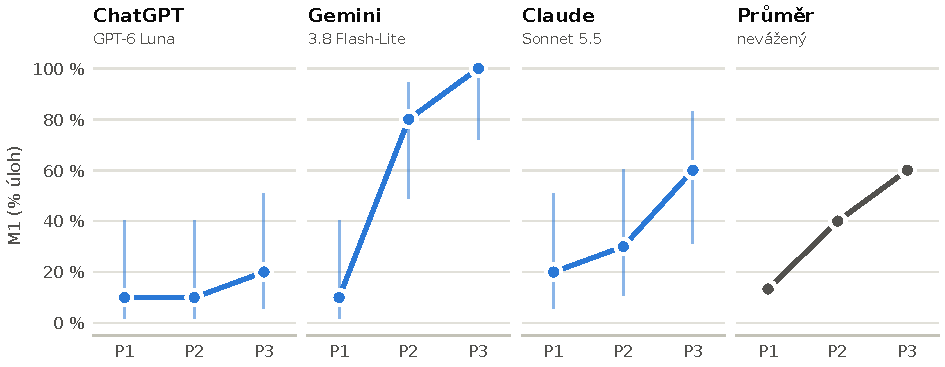
\includegraphics[width=\linewidth]{vystupy/graf_m1.pdf}
\caption{M1 podle systému a~podmínky promptu na testovací sadě. Body jsou podíly úloh s~úplnou a~přesnou množinou podob, svislé úsečky 95\% Wilsonovy intervaly. Průměr systémů je nevážený a~bez intervalu.}
\label{fig:m1}
\end{figure}

\begin{figure}[htbp]
\centering
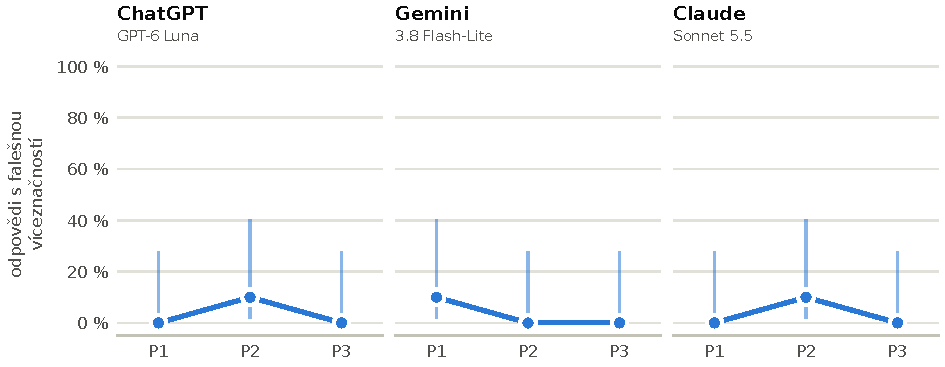
\includegraphics[width=\linewidth]{vystupy/graf_falesne.pdf}
\caption{Podíl odpovědí, v~nichž systém označil za víceznačné slovo, které víceznačné není, s~95\% Wilsonovými intervaly. Odpovědi vyřazené pro chybu formátu se sem nepromítají.}
\label{fig:falesne}
\end{figure}

\begin{figure}[htbp]
\centering
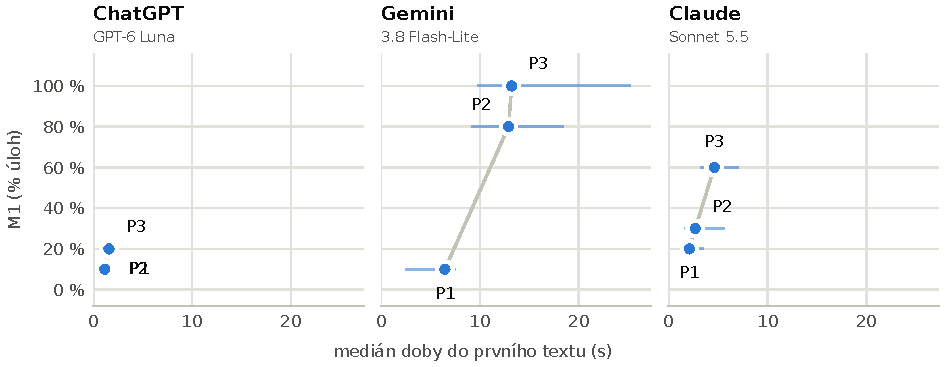
\includegraphics[width=\linewidth]{vystupy/graf_latence.pdf}
\caption{Kvalita a~rychlost: M1 proti mediánu doby do prvního textu odpovědi. Vodorovné úsečky jsou mezikvartilová rozpětí. Intervaly pro M1 jsou na obrázku~\ref{fig:m1}.}
\label{fig:latence}
\end{figure}



% ---------------------------------------------------------------------
\section{Analýza chyb}
\label{sec:analyza-chyb}

Neúspěšné odpovědi jsme podle automatické diagnostiky vyhodnocovacího
skriptu roztřídili do čtyř skupin (tabulka~\ref{tab:typy-chyb}):
\emph{neoznačená víceznačnost} (systém tiše zvolil jedinou podobu),
\emph{chybné podoby} (závorka chybí správnou podobu nebo obsahuje
nesprávnou), \emph{porušení formátu} (text navíc, více verzí věty,
stejná podoba v~závorce dvakrát nebo podoby lišící se i~jinak než
diakritikou) a~\emph{falešná víceznačnost} (závorka u~slova, které
víceznačné není). Následně jsme ručně rozebrali deset případů, mezi
nimiž jsou úspěšné i~neúspěšné výstupy všech tří systémů.

\begin{table}[htbp]
\centering
\small
\caption{Výsledek M1 a~hlavní příčina neúspěchu (30~odpovědí na systém,
všechny podmínky promptu dohromady)}
\label{tab:typy-chyb}
\begin{tabular}{@{}lccc@{}}
\toprule
 & ChatGPT & Gemini & Claude \\
\midrule
Úspěch (M1 = 1)               & 4  & 19 & 11 \\
Neoznačená víceznačnost       & 14 & 9  & 7  \\
Chybné podoby v~závorce       & 4  & 1  & 1  \\
Porušení formátu              & 8  & 1  & 11 \\
\midrule
z~toho s~falešnou víceznačností & 1 & 1 & 1 \\
\bottomrule
\end{tabular}
\end{table}

\paragraph{Případ 1: dvě víceznačná slova ve větě (test03, úspěch).}
Vstup \enquote{\dots{} nulova tolerance kanabinoidu \dots{} by urcite
zustala zachovana \dots} obsahuje dvě nezávislá víceznačná místa.
Gemini a~Claude s~optimalizovaným promptem odpověděly
\texttt{[kanabinoidu|kanabinoidů]} i~\texttt{[zachována|zachovaná]}.
ChatGPT ve všech třech podmínkách obě místa vyřešil tiše
(\enquote{kanabinoidů}, \enquote{zachována}). Gemini se strukturovaným
promptem označil jen druhé místo, Claude s~výchozím jen první. Delší
věta s~více místy je tak pro systémy obtížnější než krátká věta
s~jedním místem; s~optimalizovaným promptem však Gemini i~Claude
označily obě místa.

\paragraph{Případ 2: tichá volba jediné podoby (test01, neúspěch).}
Slovo \enquote{statu} ve spojení \enquote{obsazení statu přistěhovalci}
může být \enquote{státu} i~\enquote{států}. ChatGPT u~tohoto slova ve
všech podmínkách napsal pouze \enquote{států} (s~optimalizovaným
promptem navíc chybně závorkoval \enquote{dobývaly}), Gemini s~výchozím promptem pouze
\enquote{státu}; každý tedy zvolil jinou podobu bez upozornění. Jde
o~nejčastější typ chyby (30 z~90 odpovědí) a~přesně o~chování, kvůli
kterému studie vznikla: výsledná věta je gramaticky správná, ale
uživatel se nedozví, že existuje i~druhé čtení. Claude se
strukturovaným a~optimalizovaným promptem i~Gemini s~optimalizovaným
odpověděly správně \texttt{[státu|států]}.

\paragraph{Případ 3: tušená víceznačnost s~vymyšlenou podobou (test05, neúspěch).}
U~věty \enquote{Na zahrade videl lisku} odpověděl ChatGPT postupně
\texttt{[lišku|lišču]}, \texttt{[lišku|lys ku]} a~\texttt{[lišku|lišků]}.
Systém tedy rozpoznal, že slovo může mít více podob, ale druhou
podobu vytvořil chybně: \enquote{lišču} není české slovo, \enquote{lys
ku} jsou dvě slova a~\enquote{lišků} je jiný pád množného čísla, který
se od vstupu liší víc než diakritikou. Správnou alternativu
\enquote{lísku} (keř líska) našel pouze Gemini se strukturovaným
a~optimalizovaným promptem. Claude ve všech podmínkách napsal jen
\enquote{lišku}. Méně častá podoba je tedy pro systémy obtížně
dostupná, i~když je běžným slovem.

\paragraph{Případ 4: vzácné slovo považované za neexistující (test09, neúspěch i~úspěch).}
Věta \enquote{Tato ohromna sila nas vsechny prekvapila} připouští
\enquote{síla} i~\enquote{sila} (množné číslo slova \emph{silo}).
Gemini se strukturovaným a~optimalizovaným promptem a~ChatGPT
s~optimalizovaným odpověděli správně \texttt{[síla|sila]}. Claude
s~optimalizovaným promptem napsal nejprve \texttt{[síla|síla]}, pak
anglicky dodal, že \enquote{sila} není slovo, a~větu zopakoval bez
závorky. Model tak aktivně vyloučil platnou, ale vzácnou podobu. Pokyn
\enquote{nevypisuj podobu bez diakritiky, pokud to není skutečné
slovo} zde mohl vést k~příliš přísnému vyřazování.

\paragraph{Případ 5: samooprava uprostřed odpovědi (test07, Claude, neúspěch).}
Se strukturovaným promptem odpověděl Claude
\texttt{Význam [bodu|bodů] nebyl [jasný|jasny].}, poté anglicky
poznamenal, že \enquote{jasny} není české slovo, a~připojil opravenou
verzi \texttt{Význam [bodu|bodů] nebyl jasný.} Poslední řádek je
správně, celá odpověď ale porušuje formát, a~je proto podle M1 i~M2
chybná. Tento vzorec (chybný začátek, komentář, druhá verze) tvoří
většinu z~11 formátových chyb Claude a~objevoval se hlavně
v~odpovědích bez fáze \enquote{přemýšlení}
(oddíl~\ref{sec:limity}). Automatická kontrola zde přísně trestá
odpověď, jejíž konečný obsah je správný; měří tedy i~schopnost
odpovědět napoprvé čistě, nejen rozpoznat víceznačnost.

\paragraph{Případ 6: stejná podoba dvakrát (test07, ChatGPT, neúspěch).}
ChatGPT se strukturovaným i~optimalizovaným promptem odpověděl
\texttt{Význam [bodu|bodů] nebyl [jasný|jasný].} Víceznačné slovo
\enquote{bodu/bodů} rozpoznal správně, ale k~jednoznačnému
\enquote{jasný} přidal závorku se dvěma totožnými podobami, což je
neplatný zápis. Podobně Claude s~optimalizovaným promptem napsal
\texttt{[síla|síla]} (případ~4). Zdá se, že pokyn \enquote{uveď všechny
podoby} vede některé systémy k~mechanickému závorkování i~tam, kde
druhá podoba neexistuje.

\paragraph{Případ 7: podoby lišící se jiným písmenem (test06, neúspěch i~úspěch).}
Věta \enquote{Mysli na me} je víceznačná v~prvním slově
(rozkaz \enquote{Mysli} / oznamovací \enquote{Myslí}). Gemini ve všech
podmínkách a~Claude s~výchozím i~optimalizovaným promptem odpověděly
správně \texttt{[Mysli|Myslí] na mě.} ChatGPT s~výchozím promptem
místo toho závorkoval jen zájmeno (\texttt{Mysli na [mě|mne].}); se
strukturovaným a~optimalizovaným promptem označil i~\texttt{[Mysli|Myslí]},
ale navíc přidal \texttt{[mě|mne]}, resp.\ \texttt{[mě|mně]}. Tyto podoby se
liší přidaným písmenem, nikoli diakritikou, a~zadání je výslovně
vylučuje. Jde o~jazykově pochopitelnou záměnu (\enquote{mě} a~\enquote{mne}
jsou rovnocenné tvary), která však ukazuje, že ChatGPT nedodržel
omezení na diakritické varianty.

\paragraph{Případ 8: vzácné podstatné jméno (test10, úspěch i~neúspěch).}
\enquote{uvidel tam spici} lze číst jako \enquote{spící} i~\enquote{špici}
(pes plemene špic). Správně \texttt{[spící|špici]} odpověděl pouze
Gemini se strukturovaným a~optimalizovaným promptem. ChatGPT třikrát
nabídl neexistující \enquote{špicí} či \enquote{špící}; Claude
s~výchozím promptem vypsal čtyři varianty včetně neslov a~pak se
opravoval, s~optimalizovaným napsal jen \enquote{spící}. Případ ukazuje
stejný problém jako případ~3: systém často tuší, ve kterém slově je
víceznačnost, ale nezná nebo nevybaví si méně častou alternativu.

\paragraph{Případ 9: falešná víceznačnost (test08 a~test05, neúspěch).}
Gemini s~výchozím promptem napsal \texttt{[Ta|Tá] kůra \dots}, Claude
se strukturovaným promptem \texttt{Na zahradě [viděl|vidél] lišku}
a~ChatGPT \texttt{jedna [věc|več]}. Ve všech případech jde o~slovo,
které víceznačné není, a~o~neexistující druhou podobu. Takové odpovědi
byly vzácné (jedna na systém), což podporuje závěr, že alternativní
vysvětlení (plošné závorkování) se v~datech výrazně neprojevilo.

\paragraph{Případ 10: šum ve vstupu (test04, M2).}
Vstup \enquote{Pivoteka je polokalk( tedy vyraz, \dots{} nikoli.}
obsahuje neuzavřenou závorku. Claude ji podle reference nahradil
čárkou, Gemini a~ChatGPT závorku zachovaly a~uzavřely. Obě opravy jsou
přijatelné a~hodnotitelé je u~M2 uznali. ChatGPT s~výchozím promptem
však chybu ze vstupu ponechal (\texttt{polokalk( tedy \dots{} nikoli.})
a~v~M2 neuspěl. Víceznačnost \texttt{[přeložena|přeložená]} přitom
správně označili Gemini (P2, P3) a~Claude (P2, P3), ChatGPT ani jednou.

\paragraph{Shrnutí.}
Hlavní slabinou ChatGPT je tichá volba jediné podoby (14 z~30 odpovědí)
a~vymýšlení neexistujících alternativ; strukturovaný ani optimalizovaný
prompt to podstatně nezměnily. Claude víceznačnost často rozpoznal, ale
neuspěl kvůli samoopravám a~textu navíc (11 z~30). Gemini chyboval
hlavně s~výchozím promptem; s~P2 a~P3 našel i~vzácné alternativy
(\enquote{lísku}, \enquote{špici}, \enquote{sila}). Napříč systémy jsou
nejobtížnější méně frekventovaná slova a~věty s~více víceznačnými
místy. Automatickou kontrolu by bylo možné doplnit o~druhou metriku,
která by hodnotila pouze poslední řádek odpovědi, a~oddělit tak
rozpoznání víceznačnosti od dodržení formátu.

% ---------------------------------------------------------------------
\section{Diskuse a~limity}
\label{sec:limity}

\paragraph{Zdroje pozorované výkonnosti.}
Výsledky odrážejí kombinaci schopnosti modelu, vlivu promptu a~vlivu
produktu (výchozí chování rozhraní, rozhodování o~\enquote{přemýšlení},
bezpečnostní vrstva, třída modelu v~bezplatné verzi). Vliv nástrojů
jsme díky návrhu s~paritou vyloučili. Vliv promptu lze oddělit
porovnáním podmínek P1--P3 u~téhož systému; schopnost modelu od vlivu
produktu naše metodika neodděluje, výsledky proto nelze číst jako
čisté měření schopností modelů.

\paragraph{Velikost vzorku.}
Každá kombinace systému a~podmínky promptu byla hodnocena na deseti
testovacích větách, každá věta byla zadána jednou. Jedna věta tak
odpovídá 10~procentním bodům a~95\% Wilsonovy intervaly jsou široké
(27,8 až 51,9~p.\,b.). Nepřekrývají se pouze intervaly ChatGPT
a~Gemini u~strukturovaného a~optimalizovaného promptu. Opakované běhy
jsme neprováděli, nejistota proto nezahrnuje kolísání odpovědí při
opětovném zadání téže věty. Testy statistické významnosti
nepoužíváme; při tak malém vzorku by měly nízkou sílu
\cite{dror2018,miller2024}. Výsledky interpretujeme podle velikosti
efektu a~intervalů nejistoty.

\paragraph{Počet a~výběr systémů.}
Místo plánovaných čtyř systémů hodnotíme tři, protože Grok se kvůli
omezením bezplatné verze nepodařilo změřit
(oddíl~\ref{sec:grok-omezeni}). Testovali jsme bezplatné webové verze
s~výchozím nastavením: ChatGPT (viditelné označení modelu GPT-6 Luna),
Gemini (3.8 Flash-Lite) a~Claude (Sonnet 5.5). Bezplatné nabídky se
liší třídou modelu, Gemini například poskytuje odlehčený model
Flash-Lite. Výsledky proto popisují srovnání produktů v~jejich
bezplatné podobě k~datu měření, nikoli schopnosti nejsilnějších modelů
daných výrobců ani samotných jazykových modelů. ChatGPT a~Gemini
běžely v~anonymním režimu, Claude v~anonymním chatu přihlášeného
bezplatného účtu, protože režim bez přihlášení nenabízí.

\paragraph{Chování produktu.}
Webové rozhraní Claude samo rozhoduje, zda před odpovědí
\enquote{přemýšlí}. Ze 30~testovacích odpovědí Claude jich 14 vzniklo
s~přemýšlením a~všechny byly jednořádkové, správně podle M1 jich bylo
9. U~16 odpovědí bez přemýšlení byly správně pouze 2; model v~nich
často napsal chybný začátek, opravu a~druhou verzi věty, což je
porušení formátu. Výsledek Claude tak silně závisí na chování
produktu, které uživatel v~bezplatné verzi neovládá.

\paragraph{Kontext konverzace.}
Věty jedné podmínky byly zadávány postupně v~jednom vlákně, pozdější
odpovědi proto mohly být ovlivněny předchozími. Ve vlákně
optimalizovaného promptu předcházelo testovací sadě u~všech systémů
30 vývojových a~validačních vět, zatímco vlákna výchozího
a~strukturovaného promptu obsahovala jen testovací věty. Část rozdílu
mezi P3 a~ostatními podmínkami proto může plynout z~delšího kontextu,
nejen ze změny promptu. U~Claude produkt po větě dev07 pozastavil
první vlákno optimalizovaného promptu (hlášení bezpečnostní vrstvy)
a~sběr pokračoval od dev08 v~novém vlákně.

\paragraph{Ladění optimalizovaného promptu.}
Optimalizovaný prompt byl laděn pro každý systém zvlášť a~s~různou
intenzitou: ChatGPT jednou úpravou (zmrazená verze~2), Gemini čtyřmi
(verze~5) a~Claude pěti (verze~6). Prompt pro Claude byl navíc laděn
s~pomocí AI asistenta. Rozdíly v~přínosu P3 mezi systémy proto
odrážejí i~rozdílné úsilí vložené do ladění. Vývojová sada má jen
20~vět, ladění na ní tedy může vést k~přeučení na konkrétní případy
\cite{perez2021}; tomu má bránit testovací sada držená stranou.

\paragraph{Konstrukce metriky M1.}
M1 vyžaduje současně správnou množinu podob a~dodržení formátu. Neúspěch
v~M1 proto nemusí znamenat, že systém víceznačnost nerozpoznal.
Porušení formátu tvořila u~Claude 4, 6 a~1 odpověď (P1, P2, P3), u~ChatGPT
2, 3 a~3 a~u~Gemini 0, 1 a~0. U~Claude jde tedy velká část neúspěchů
s~P1 a~P2 na vrub formátu, u~ChatGPT naopak převažují chybějící nebo
nesprávné podoby slov. Podobně M2 hodnotí odpověď porušující formát
jako chybnou, což vysvětluje nízké M2 Claude u~strukturovaného promptu
(30~\%).

\paragraph{Měření latence.}
Doba do prvního textu odpovědi (M3) byla měřena skriptem v~konzoli
prohlížeče. Pro ChatGPT a~Gemini jsme použili společný měřicí skript,
pro Claude upravenou verzi, která ignoruje indikátory přemýšlení
a~popisky rozhraní. Měření proto nejsou mezi systémy plně srovnatelná
a~závisí také na připojení a~vytížení služby. U~Gemini (P1) nesouhlasí
čas odeslání věty test07 s~dobou odpovědi na test06. U~ChatGPT (P1)
byla odpověď na test06 přerušena odesláním další zprávy; hodnotíme ji
v~podobě, v~jaké byla zaznamenána. Časy z~vývojových a~validačních běhů
Claude nejsou spolehlivé a~do výsledků nevstupují.

\paragraph{Reference a~lidské hodnocení.}
Datovou sadu, referenční věty i~lidské hodnocení vytvořili členové
řešitelského týmu; reference schválil jeden člen týmu. Hodnotitelé
neznali identitu systému ani podmínku promptu, znali však cíl studie.
Rubrika M2 byla po prvním průchodu upřesněna
(oddíl~\ref{sec:lidske-hodnoceni}). Část vět pochází z~veřejně dostupných
dat, s~nimiž se hodnocené systémy mohly setkat při trénování
(oddíl~\ref{sec:data}).

% ---------------------------------------------------------------------
\section{Závěr}
\label{sec:zaver}

Na testovací sadě deseti vět se tři hodnocení asistenti výrazně lišili
v~tom, jak úspěšně v~české větě bez diakritiky rozpoznají víceznačné
slovo a~uvedou přesně všechny jeho podoby. Rozdíly navíc silně závisely
na podmínce promptu. Gemini dosáhl s~výchozím promptem 1, se
strukturovaným 8 a~s~optimalizovaným 10 správných odpovědí z~10,
Claude 2, 3 a~6 a~ChatGPT 1, 1 a~2.

Hypotéza, že strukturovaný prompt zvýší M1, je v~datech formálně
podpořena: průměrná změna činí $+$26,7~p.\,b. a~zlepšení nastalo
u~dvou ze tří systémů. Podpora je však slabá. Téměř celý průměrný
efekt pochází z~Gemini ($+$70~p.\,b.). U~Claude odpovídá zlepšení
o~10~p.\,b. čistému rozdílu jediné věty (3 věty se zlepšily, 2
zhoršily) a~u~ChatGPT se M1 nezměnila. Optimalizovaný prompt zvýšil
M1 oproti strukturovanému u~všech tří systémů (o~10 až 30~p.\,b.),
jeho přínos však nelze oddělit od delšího kontextu vlákna a~rozdílného
úsilí při ladění. Alternativní vysvětlení, tedy plošné označování slov
za víceznačná, se v~datech výrazně neprojevilo: odpovědí se závorkou
u~slova, které víceznačné není, bylo nejvýše 2 z~30 na podmínku.

Strukturovaný prompt byl pro všechny systémy shodný, optimalizované
verze se lišily (1 až 5 úprav specifických pro systém) a~měly 3114 až
5504 znaků oproti 763 znakům výchozího promptu. Prompt, který výrazně
pomohl jednomu systému, tedy nemusí stejně pomoci ostatním: u~ChatGPT
nezlepšil strukturovaný prompt M1 vůbec a~chyby zůstávaly převážně
obsahové, nikoli formátové.

Vyšší přesnost přitom nebyla zadarmo. Gemini s~nejlepším skóre měl
také nejdelší dobu do prvního textu odpovědi (medián 13,2~s
s~optimalizovaným promptem), zatímco ChatGPT odpovídal nejrychleji
(1,3 až 1,6~s) s~nejnižší úspěšností. Metriky neslučujeme do jednoho
skóre; Pareto-frontu kombinací, které nejsou v~M1 i~M3 současně
překonány jinou kombinací, tvoří ChatGPT (P2, P3), Claude (P2, P3)
a~Gemini (P2, P3). Výsledky platí pro bezplatné webové
verze hodnocených produktů, pro tento typ úlohy a~pro období měření
(říjen 2026). Vzhledem k~velikosti vzorku je považujeme za předběžné
pozorování, nikoli za doklad obecné převahy některého systému.



% ---------------------------------------------------------------------
\begin{thebibliography}{99}

\bibitem{cohen1960}
J.~Cohen. A coefficient of agreement for nominal scales.
\emph{Educational and Psychological Measurement}, 20(1):37--46, 1960.

\bibitem{dror2018}
R.~Dror, G.~Baumer, S.~Shlomov, R.~Reichart. The Hitchhiker's Guide to
Testing Statistical Significance in Natural Language Processing.
In \emph{Proceedings of ACL}, 2018.

\bibitem{miller2024}
E.~Miller. Adding Error Bars to Evals: A Statistical Approach to
Language Model Evaluations. arXiv:2411.00640, 2024.

\bibitem{mizrahi2024}
M.~Mizrahi, G.~Kaplan, D.~Malkin, R.~Dror, D.~Shahaf, G.~Stanovsky.
State of What Art? A Call for Multi-Prompt LLM Evaluation.
\emph{Transactions of the Association for Computational Linguistics},
12, 2024.

\bibitem{naplava2018}
J.~Náplava, M.~Straka, P.~Straňák, J.~Hajič. Diacritics Restoration
Using Neural Networks. In \emph{Proceedings of LREC}, 2018.

\bibitem{naplava2021}
J.~Náplava, M.~Straka, J.~Straková. Diacritics Restoration using BERT
with Analysis on Czech language. \emph{The Prague Bulletin of
Mathematical Linguistics}, 116, 2021. arXiv:2105.11408.

\bibitem{perez2021}
E.~Perez, D.~Kiela, K.~Cho. True Few-Shot Learning with Language Models.
In \emph{Advances in Neural Information Processing Systems}, 2021.

\bibitem{sclar2024}
M.~Sclar, Y.~Choi, Y.~Tsvetkov, A.~Suhr. Quantifying Language Models'
Sensitivity to Spurious Features in Prompt Design or: How I~learned to
start worrying about prompt formatting. In \emph{Proceedings of ICLR},
2024.

\bibitem{wilson1927}
E.~B.~Wilson. Probable inference, the law of succession, and statistical
inference. \emph{Journal of the American Statistical Association},
22(158):209--212, 1927.

\end{thebibliography}

\end{document}